Typical real world clustering problems can have subjective clustering numbers. For this reason, an experiment was done to determine the rand index for all integers in $[2,10]$ cluster means in order to determine the optimal cluster amount which represents our particular skewed MNIST dataset. Using the histogram in figure~6, we can estimate the appropriate amount of clusters which would perform the highest Rand Index, and determine the validity of our hypothesis with our experiment. Given the results discussed in the results section, it appears that four clusters in the PCA representation and 3 clusters in the fully dimensioned representation of the skewed MNIST gave the best rand index score, even though ten unique labels were used in the truth labels. In the future, this experiment can be run with different skewed representations of the MNIST dataset to determine if the results are consistent. \par

\begin{figure}[H]
    \centering
    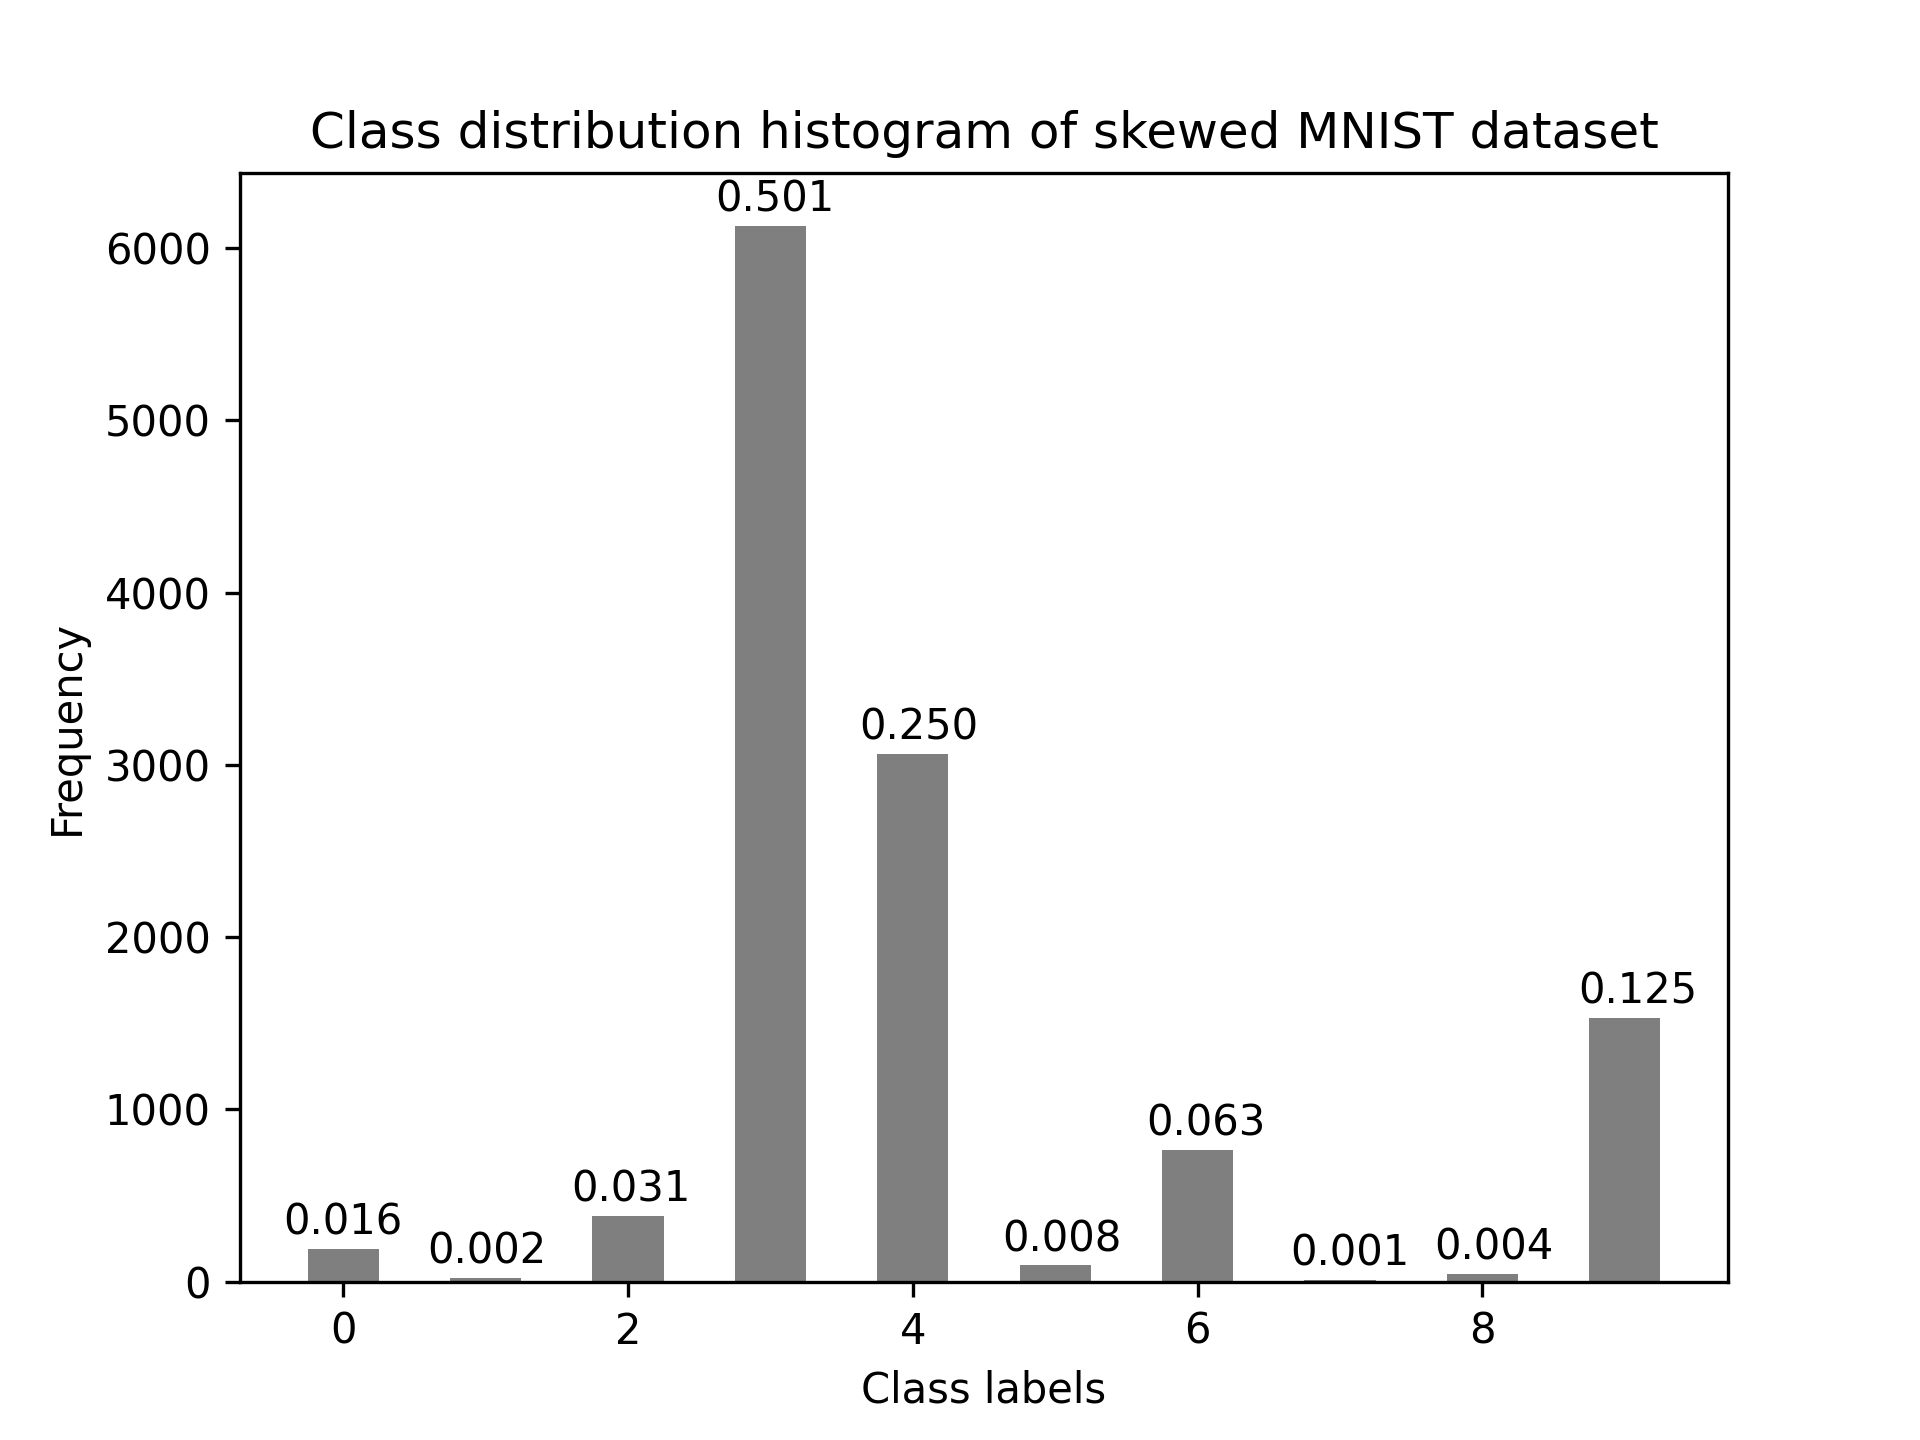
\includegraphics[width=0.45\textwidth]{class_histogram.png}
    \caption{Class Representation in Skewed MNIST Dataset\label{fig:hist1}}    
\end{figure}

Additionally, consideration must be taken regarding the rand index metric on a soft clustering algorithm like FCM. The implementation of the rand index in this assignment took the maximum probability a point would be within a given $k^{th}$ cluster, and then implemented the rand index as described in the methods section. The rand index calculates the similarities of points in different clusters as a fixed yes or no. As FCM is a soft clustering algorithm, the probabilities of points being within all clusters are returned, therefore a different metrics could potentially give more insight to the accuracy of soft clustering algorithms. \par

Lastly, two representations of the data was evaluated: PCA and Scaled. PCA scales down the dimensionality of the data to two dimensions which theoretically decreases the complexity, but also hinders the accuracy of the clustering method. In this implantation, the reduction of accuracy was only one percent, which inclines us to believe that the PCA representation would be sufficiently similar to a fully dimensional representation on a larger dataset with similar skewed ratios. \par